\section{Implementazione del database}
Nelle sezioni precedenti si è discusso delle proprietà
offerte dai diversi tipi di database e
delle necessità che il dominio impone sul sistema.
La scelta del database deriva quindi dall'incrocio di tutte queste condizioni,
individuando la tecnologia che meglio riesce a rispondere alle esigenze del progetto.
Ogni tipologia di database comporta un approccio differente alle informazioni,
implicando una strategia di salvataggio e manipolazione dei dati propria.
Le strutture che modellano le entità devono quindi
essere create per sfruttare nella maniera più efficiente possibile
i vantaggi offerti dalla tecnologia scelta.\\
\\
Una volta scelto il database e le strutture in base alla modalità
che più si addicono alle esigenze del progetto,
l'utilizzo di servizi in cloud comporta una maggiore attenzione anche
alle proprietà legate al mantenimento del servizio,
dalle quali derivano le proprietà di scalabilità e affidabilità.
La grande differenza tra i vari servizi sta nelle proprietà del server
incaricato di fornire il potere computazionale necessario per l'esecuzione.
L'architettura del server e la sua integrazione con la tecnologia del database
determinano infatti l'effettiva capacità di scalabilità del servizio.\\
\\
Si intende scalabilità verticale la capacità di aumentare le risorse
della stessa macchina in cui si esegue il codice.
La scalabilità verticale viene definita nel momento di creazione del servizio,
in cui si determinano le risorse da dedicare alla macchina che esegue il programma.
Trattandosi di macchine virtualizzate,
è sempre possibile in un secondo momento aumentare le prestazioni in caso di necessità.\\
\\
Per scalabilità orizzontale si intende invece la capacità di
delegare il carico di lavoro su più macchine, eventualmente coordinando le modifiche.
Questo permette una risposta alle richieste più resistente,
riducendo il rischio di colli di bottiglia che potrebbero venirsi a formare nell'utilizzo di un nodo singolo.
La scalabilità orizzontale richiede però l'implementazione
di tecnologie apposite integrate con il database che permettano l'esecuzione in nodi fisici differenti. \\
\\
Una volta individuata la tecnologia adatta e il livello di scalabilità desiderati,
è bene considerare le altre necessità o le opportunità aggiuntive generate
dalla presenza di un database nel progetto. \\
\\
L'alta disponibilità(HA) è la proprietà di garantire l'accesso al servizio nonostante i guasti.
Ad esempio, si può mantenere una macchina identica al server principale in grado di replicare il servizio,
spostando il carico in caso di guasto del server principale.
Si misura in “numero di nove”, ovvero la quantità di nove presenti
nella percentuale del tempo per il quale si garantisce la disponibilità del servizio.
I servizi offrono diverse qualità di HA, in base alle funzionalità desiderate.\\
\\
Alcuni servizi possono presentare offerte di backup
per riportare il server nello stesso stato di qualche momento precedente.
Questo permette il ripristino del sistema a un punto precedente
rispetto all'avvenimento di eventuali errori o guasti del sistema.

\subsection{Scelta del database}

Viste le necessità del progetto in ambito di scalabilità
e le caratteristiche del dominio,
si individua nei database documentali la tecnologia più adatta
per gestire la persistenza centrale dell'applicazione.\\
\\
I database documentali, facenti parte della categoria dei database non relazionali,
rappresentano un paradigma di gestione dei dati
che organizza le informazioni in documenti.
Ogni documento è un'unità autonoma che incapsula la descrizione di un'entità,
contenendo le sue proprietà.
Tali documenti sono logicamente raggruppati in collezioni.
All'interno di una collezione,
ciascun documento è univocamente individuato da un proprio identificativo,
garantendo l'accesso e la manipolazione diretta.\\
\\
Un aspetto distintivo e strategicamente rilevante dei database documentali è
la loro intrinseca capacità di supportare la scalabilità orizzontale in modo nativo.
Data la natura dei documenti e il loro accoppiamento debole con gli altri elementi,
la separazione delle collezioni risulta particolarmente semplificata,
favorendo un partizionamento dei dati,
essenziale per distribuire il database su diversi nodi fisici di archiviazione.
Questo vantaggio è fondamentale in architetture distribuite e ambienti ad alta intensità di dati.\\
\\
Un altra caratteristica derivata dall'utilizzo di un database non relazionale
è la propensione verso la denormalizzazione degli elementi del dominio,
sia strutturale che logica.
Vista la difficoltà intrinseca nell'ottimizzare le join tra documenti,
che comporta una minore efficienza nell'operazione di incrocio tra entità,
si propende, invece che a incrociare i dati, a duplicarli sui vari documenti.
La denormalizzazione consiste infatti nel riportare 
le stesse proprietà di alcuni elementi in più collezioni.\\
\\
Se correttamente ottimizzata, 
il numero necessario di join o di richieste al database 
per soddisfare le esigenze viene notevolmente ridotto.
Le operazioni di join sono così agevolate,
in quanto possono essere ottimizzate per
far risiedere la risorsa voluta all'interno dello stesso documento 
o della stessa partizione dell'elemento di partenza,
minimizzando la necessità di operazioni di giunzione o di lettura di tabelle tra nodi distinti.
Questo necessita di aggregare i dati attorno agli elementi chiave su cui vertono le richieste,
favorendo la divisione dei dati anche in caso di relazioni complesse.\\
\\
La denormalizzazione comporta intrinsecamente
alcune sfide a livello di consistenza dei dati,
in particolare per le operazioni di modifica che coinvolgono informazioni duplicate.
Infatti, pur se si modificasse atomicamente il documento direttamente coinvolto dalla modifica,
bisognerebbe comunque aggiornare tutte le altre parti che includono quella proprietà.
Oltre a dover progettare l'applicazione affinché sia resiliente all'inconsistenza temporanea - ad esempio mostrando dati "vecchi" per un breve periodo prima che le modifiche vengano propagate
o implementando logiche di compensazione che possano correggere eventuali discrepanze -
è necessario implementare la logica per garantire che la modifica venga propagata correttamente.\\
\\
Esistono diverse strategie che consentono gestire le informazioni duplicate
in modo efficace, mitigandone l'impatto.
Una delle soluzioni avviene direttamente tramite trigger a livello di database,
che scatena la chiamata per correggere i dati ove necessario.
Un altro modo consiste nelle code di messaggistica.
Questo prevede un orchestratore per la distribuzione degli aggiornamenti,
che riceve notifiche delle variazioni.
Un secondo processo le elabora per poi applicare le modifiche.
Un'altra tecnica ancora risiede in servizi eseguiti in background,
che periodicamente scansionano e sincronizzano i dati.
Infine, si possono adottare timestamp o numeri di versione
su ciascun documento o campo denormalizzato,
permettendo alle applicazioni di determinare la versione più recente di un dato,
risolvendo i conflitti quando si presentano aggiornamenti concorrenti o ritardati.\\
\\
Implementando automaticamente e nativamente la scalabilità orizzontale,
un database non relazionale ci permette di gestire con efficienza
l'incremento dei volumi di dati e dei carichi di lavoro 
senza l'attuazione di interventi complessi.
Fornisce inoltre un supporto diretto all'esigenza del dominio di Wyd
riguardo alla necessita di letture performanti
da entrambi i lati di relazioni molti-a-molti:
attraverso un partizionamento strategico,
i dati correlati possono essere collocati in partizioni vicine,
ottimizzando le letture da entrambi i lati della relazione.
Infine, un'attenta progettazione del modello di dati,
- che include una denormalizzazione strategica e l'utilizzo degli indici -
garantisce un tempo di recupero delle informazioni ridotto,
massimizzando la reattività del sistema e l'efficienza complessiva.\\
\\
Un confronto con il paradigma relazionale evidenzia le ragioni
della sua esclusione per le esigenze del nostro progetto.
Sebbene i database relazionali siano soluzioni consolidate per la gestione di dati strutturati,
presentano delle limitazioni che non si allineano con i requisiti di scalabilità richiesti.
La capacità di garantire le proprietà ACID necessita 
di un controllo sulle transazioni,
limitando il numero massimo di connessioni simultanee che possono essere gestite.
Questo influenza l'abilità di rispondere a un numero massiccio di richieste contemporanee.\\
\\
Inoltre, la loro architettura non prevede la separazione fisica degli schemi in relazione tra loro,
legandoli alla stessa partizione logica.
Questo impone intrinsecamente dei vincoli sulla scalabilità orizzontale,
in quanto l'implementazione dello sharding, sebbene possibile,
viene lasciata interamente a carico dello sviluppatore,
introducendo un significativo onere di progettazione, sviluppo e manutenzione.\\
\\
La gestione di relazioni molti-a-molti nel modello relazionale
si pone infatti in diretto contrasto con la denormalizzazione dei dati,
utilizzando un'unica tabella di giunzione per descriverne il rapporto.
Se si decidesse di distribuire gli schemi relazionali su più partizioni,
la divisione della tabella di giunzione introdurrebbe svantaggi prestazionali,
indipendentemente dalla strategia usata.
Se si separasse la tabella in base a uno degli elementi che unisce
verrebbe compromessa l'abilità di ritrovare i dati a partire 
da uno degli altri elementi e viceversa:
per quanto sarebbero disponibili tutti i dati di un elemento 
dell'associazione sulla sua stessa partizione
- sfruttando al massimo la velocità di unione tra schemi dei relazionali -
per eseguire la ricerca in senso inverso bisognerebbe invece
allargare la richiesta a tutte le partizioni del sistema.
In un ambiente distribuito e con volumi di dati in crescita,
le join richiedono quindi l'analisi e il trasferimento di grandi quantità di dati tra nodi diversi,
riducendo le performance complessive.
Questi fattori combinati ci hanno portato a escludere il modello relazionale.\\
\begin{figure}[h!]
    \centering
    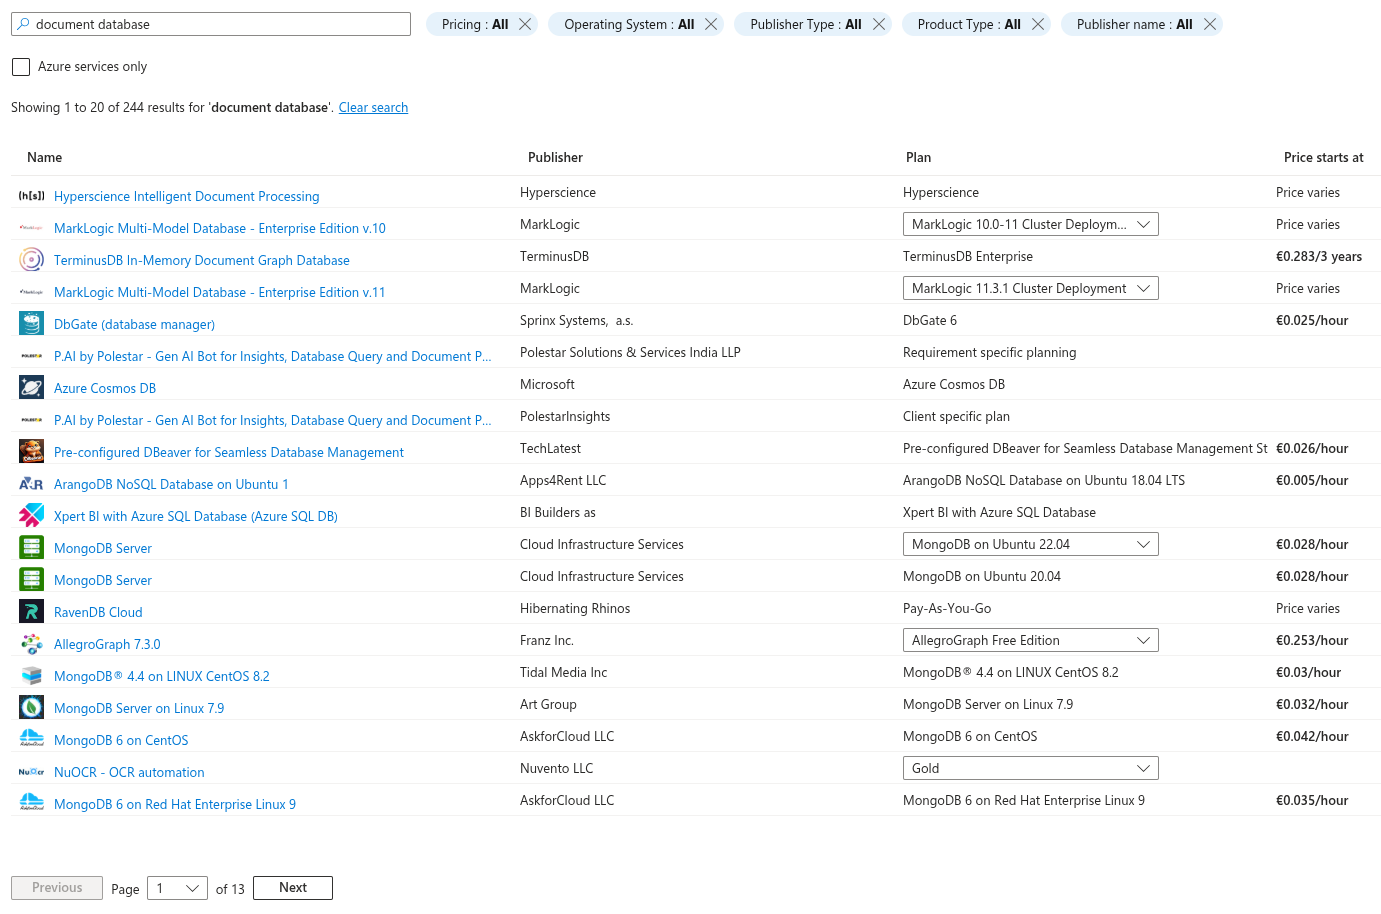
\includegraphics[width=\textwidth]{AzureDatabase.png}
    \caption{Proposte di Azure per i database documentali}
\end{figure}
\\
Essendo il progetto già improntato su Azure,
la ricerca verte inizialmente tra le opzioni che  la piattaforma mette a disposizione.
Azure offre un'ampia scelta di database documentali
che possono essere integrati con il resto dell'ecosistema.
Tuttavia, Azure presenta un servizio nativo per i database non relazionali
completamente gestito, chiamato Azure Cosmos DB.
Garantendo la massima interoperabilità all'interno dell'ecosistema,
si procede analizzando le proprietà e i vantaggi offerti da Cosmos DB.\\
\begin{wrapfigure}{o}{0.25\textwidth}
    \centering
    
\includegraphics[height=.12\textheight]{cosmos.png}
    Azure Cosmos
\end{wrapfigure}
Azure Cosmos DB si distingue per la sua capacità di scalare orizzontalmente in maniera illimitata,
consentendo di gestire volumi di dati e carichi di lavoro molto elevati,
fino a milioni di richieste al secondo,
grazie alla possibilità di distribuire il carico su più regioni Azure.
È stato infatti ideato per presentare un'architettura distribuita,
con replica automatica dei dati,
assicurando un'elevatissima disponibilità e resilienza.
Queste vengono assicurate anche in caso di interruzioni regionali,
grazie a meccanismi di failover automatico.
Inoltre, la distribuzione globale garantisce che i dati siano sempre vicini agli utenti,
riducendo drasticamente la latenza a millisecondi
(con SLA del 99.999\% di disponibilità per account multi-regione).
Consente l'indicizzazione attraverso più partizioni in maniera automatica e personalizzabile, ottimizzando le query, riducendo la complessità e migliorando le prestazioni,
senza richiedere oneri di gestione manuale degli indici.\\
\\
Pur essendo focalizzato sui database documentali,
Cosmos DB è però una soluzione multi-modello e multi-API.
Supporta infatti, oltre alla sua API nativa per NoSQL (che usa il modello a documenti JSON),
anche API compatibili con MongoDB, Apache Cassandra, Apache Gremlin (per i grafi) e Azure Table.
Questa versatilità permette agli sviluppatori di utilizzare strumenti  a loro familiari,
semplificando la migrazione di applicazioni esistenti o
lo sviluppo di nuove con la flessibilità di scegliere il modello di dati più appropriato.\\
\\
A livello di costi è difficile portare un'analisi precisa,
in quanto tutti i competitor presentano servizi
con capacità, disponibilità e integrazione differenti.
I modelli di pagamento si basano su metriche di utilizzo diverse,
rendendo necessarie ulteriori analisi che dipendono anche
dall'effettiva tipologia e quantità di richieste che vertono sul database.
Di seguito viene riportata una tabella per comparare i costi delle alternative principali.
Cosmos usa come metrica le Request Unit (RU)
per quantificare l'impatto di una richiesta sul database.
Le RU rappresentano un'astrazione delle risorse di sistema (CPU, I/O, memoria).
Ogni operazione consuma RU, proporzionalmente alla sua
complessità, dimensione e al carico computazionale richiesto.\\

\begin{longtable}{|P{3.2cm}|P{4.2cm}|P{4.2cm}|P{3cm}|}
    \hline
    \textbf{Servizio}      & \textbf{Costo ogni milione di scritture}\newline(normalizzate a 1 KB) & \textbf{Costo ogni milione di scritture}\newline (normalizzate a 1 KB) & \textbf{Costo di manutenzione GB/mese} \\
    \hline
    \endhead
    AWS DynamoDB           & \$1.25                                                                & \$0.25                                                                 & \$0.25                                 \\
    \hline
    Google Cloud Firestore & \$0.90                                                                & \$0.30                                                                 & \$0.156                                \\
    \hline
    Azure Cosmos DB        & In base al consumo di RU, \$5.84 al mese ogni 100RU/s                 & In base al consumo di RU, \$5.84 al mese ogni 100RU/s                  & \$0.25 (Transazionale)                 \\
    \hline
    \caption{Costi dei principali database documentali gestiti in Cloud}
\end{longtable}

La difficoltà di stabilirne il costo in una fase iniziale
è mitigata però dalla presenza di un piano gratuito perenne.
Cosmos DB offre infatti una quota gratuita di risorse iniziali,
per tutta la durata dell'utilizzo.
Il piano prevede 25 GigaByte di memoria gratuita,
a cui si aggiungono 1000 RU/s offerti per ogni categoria di operazione,
suddivise in lettura, scrittura ed eliminazione.
Dato lo stadio iniziale del progetto,
queste caratteristiche sono state considerate sufficienti,
permettendo di sfruttare e testare le sue capacità di distribuzione.\\
\\
Nel caso in cui da un'analisi condotta durante fasi successive del progetto
- sfruttando dati derivati dall'utilizzo effettivo dell'applicazione -
emerga che Cosmos DB non rappresenti l'opzione più adeguata,
lo spostamento dei dati verso un altro gestore comporterà uno sforzo limitato (ma non un costo),
data la compatibilità nella rappresentazione dei dati
tra le diverse tecnologie di database documentali.

\subsection{Configurazione di Cosmos DB}

La creazione di una nuova istanza di Cosmos DB
richiede la definizione delle impostazioni di funzionamento,
che ne determinano le proprietà a livello di 
disponibilità, ridondanza, sicurezza e resilienza ai guasti.\\
\\
La prima impostazione riguarda la distribuzione geografica dei dati.
Cosmos distribuisce sue risorse su entità nominate zone, che vengono raggruppate in regioni.
L'opzione di usare delle availability zones duplica i dati
su più zone all'interno della stessa regione.
Questo crea ridondanza dei dati per una maggiore resistenza ai guasti,
e così facendo aumenta la disponibilità dei dati,
che,
partendo da un disponibilità garantita iniziale per la zona singola del 99.99\% (sulle scritture),
risulta pari a 99.995\%.
Si evita così la perdita dei dati e delle funzionalità
in caso una zona non sia più raggiungibile.
L'aggiunta di ulteriori regioni diminuirebbe il rischio indisponibilità a causa di guasti
(i dati verrebbero duplicati anche tra le varie regioni),
ma aumenterebbe la complessità generale e il costo dell'applicazione.
Nella fase iniziale si è optato per garantire una ridondanza a livello di zone,
selezionando quindi l'opzione delle availability zones,
ma rimanendo all'interno di una singola regione.\\

\begin{figure}[h!]
    \centering
    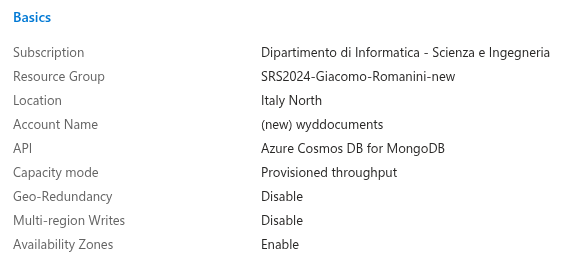
\includegraphics[width=\textwidth]{cosmosbasics.png}
    \caption{Impostazioni generali di Azure Cosmos DB}
\end{figure}

Volendo inizialmente rimanere in una singola regione,
l'impostazione "Geo-Redundancy" non è stata abilitata.
Allo stesso modo le scritture su più regioni non sono state abilitate,
preferendo un approccio centralizzato.\\
\\
Come modello di costo Azure propone due modalità distinte: serverless e provisioned throughput.
Nella modalità serverless il servizio scala in base alle richieste,
e viene quindi considerato solo l'effettivo utilizzo di risorse usate.
Adatto a carichi di richieste improvvisi e sbilanciati,
non supporta l'esecuzione su più regioni.
Il provisioned throughput richiede invece una previsione delle risorse necessarie,
per metterle a disposizione e farsi pagare di conseguenza, che siano state usate o meno.
Questo necessita quindi di una stima del carico previsto,
per poi impostare le risorse.
Azure permette di affiancargli l'opzione autoscale,
la cui funzionalità consiste nel modificare automaticamente
(all'interno di un intervallo predefinito)
le risorse messe a disposizione in base al carico del momento,
per poi considerare il massimo valore raggiunto in quell'ora.
Questo permette di evitare l'implementazione di una strategia di allocazione delle risorse,
mantenendo comunque i costi legati al consumo effettivo delle risorse.\\
\\
Prevedendo un carico di richieste non troppo elevato,
ma anche costante e poco variegato,
e considerando il minor tempo di latenza medio e il supporto a multiple regioni,
si è scelta una strategia di pagamento di tipologia provisioned throughput,
con l'opzione autoscale che verrà poi impostata, 
per sfruttare comunque la scalabilità del servizio,
su un intervallo di risorse inizialmente contenuto.\\
\\
Per migliorare la sicurezza del database e garantire il controllo degli accessi,
il database è stato inserito all'interno di una rete virtuale privata.
Si isola così il sistema da tutti gli attori esterni alla rete,
limitando l'accesso ai soli altri nodi che ne fanno parte.
Verranno quindi aggiunti alla rete solo i servizi che devono comunicare con Cosmos DB,
in particolare Azure Functions e il Key Vault 
(che contiene le chiavi per la cifratura dei dati).
La ridondanza tra le varie zone garantisce il ritrovamento dei dati
anche in caso di indisponibilità di un'istanza del database,
ma si è scoperti qualora vengano apportate modifiche erronee o malintenzionate 
che richiedano il ripristino dei dati a uno stato precedente.\\
\\
Il servizio di backup proposto da Azure permette di salvare
lo stato dei dati fino a un certo momento nel passato,
in maniera da garantire il ritorno a una situazione precedente
nel caso in cui ci si accorga siano state effettuate modifiche non desiderate.
Azure permette di configurare la tipologia di backup, 
sia seguendo delle opzioni preimpostate,
che personalizzandola in termini di durata, grandezza dei salvataggi e numero di copie.
Nel nostro caso si è scelto di applicare il servizio incluso gratuitamente
che mantiene le modifiche avvenute negli ultimi sette giorni.

\clearpage

\subsection{Definizione delle collezioni}

Stabiliti la tipologia e il comportamento del servizio che ospita il database,
bisogna definire la struttura il cui le classi vengono salvate,
in maniera da sfruttare al meglio le sue proprietà,
allineando i dati alle procedure di lettura e scrittura,
per ottimizzare il carico e il tempo di risposta.\\
\\
Grazie alle proprietà di accoppiamento debole e al supporto alla denormalizzazione delle entità,
la libertà di modellazione del dominio fornita da Cosmos DB è massima.
Partendo dalle entità principali, a ognuna di esse è stata associata una collezione.
Sono state così definite le entità di User, Profile, Event, Image e Group,
che rispondono agli omonimi elementi del dominio.
A Event e Profile si aggiungono ProfileDetails ed EventDetails,
che contengono i dati particolari di questi elementi.
Gli Account sono gestiti internamente da Firebase Authentication,
e la loro relazione con gli utenti è stata mappata in un insieme all'interno di User
tramite i loro Uid.\\
\begin{figure}[htbp]
    \centering
    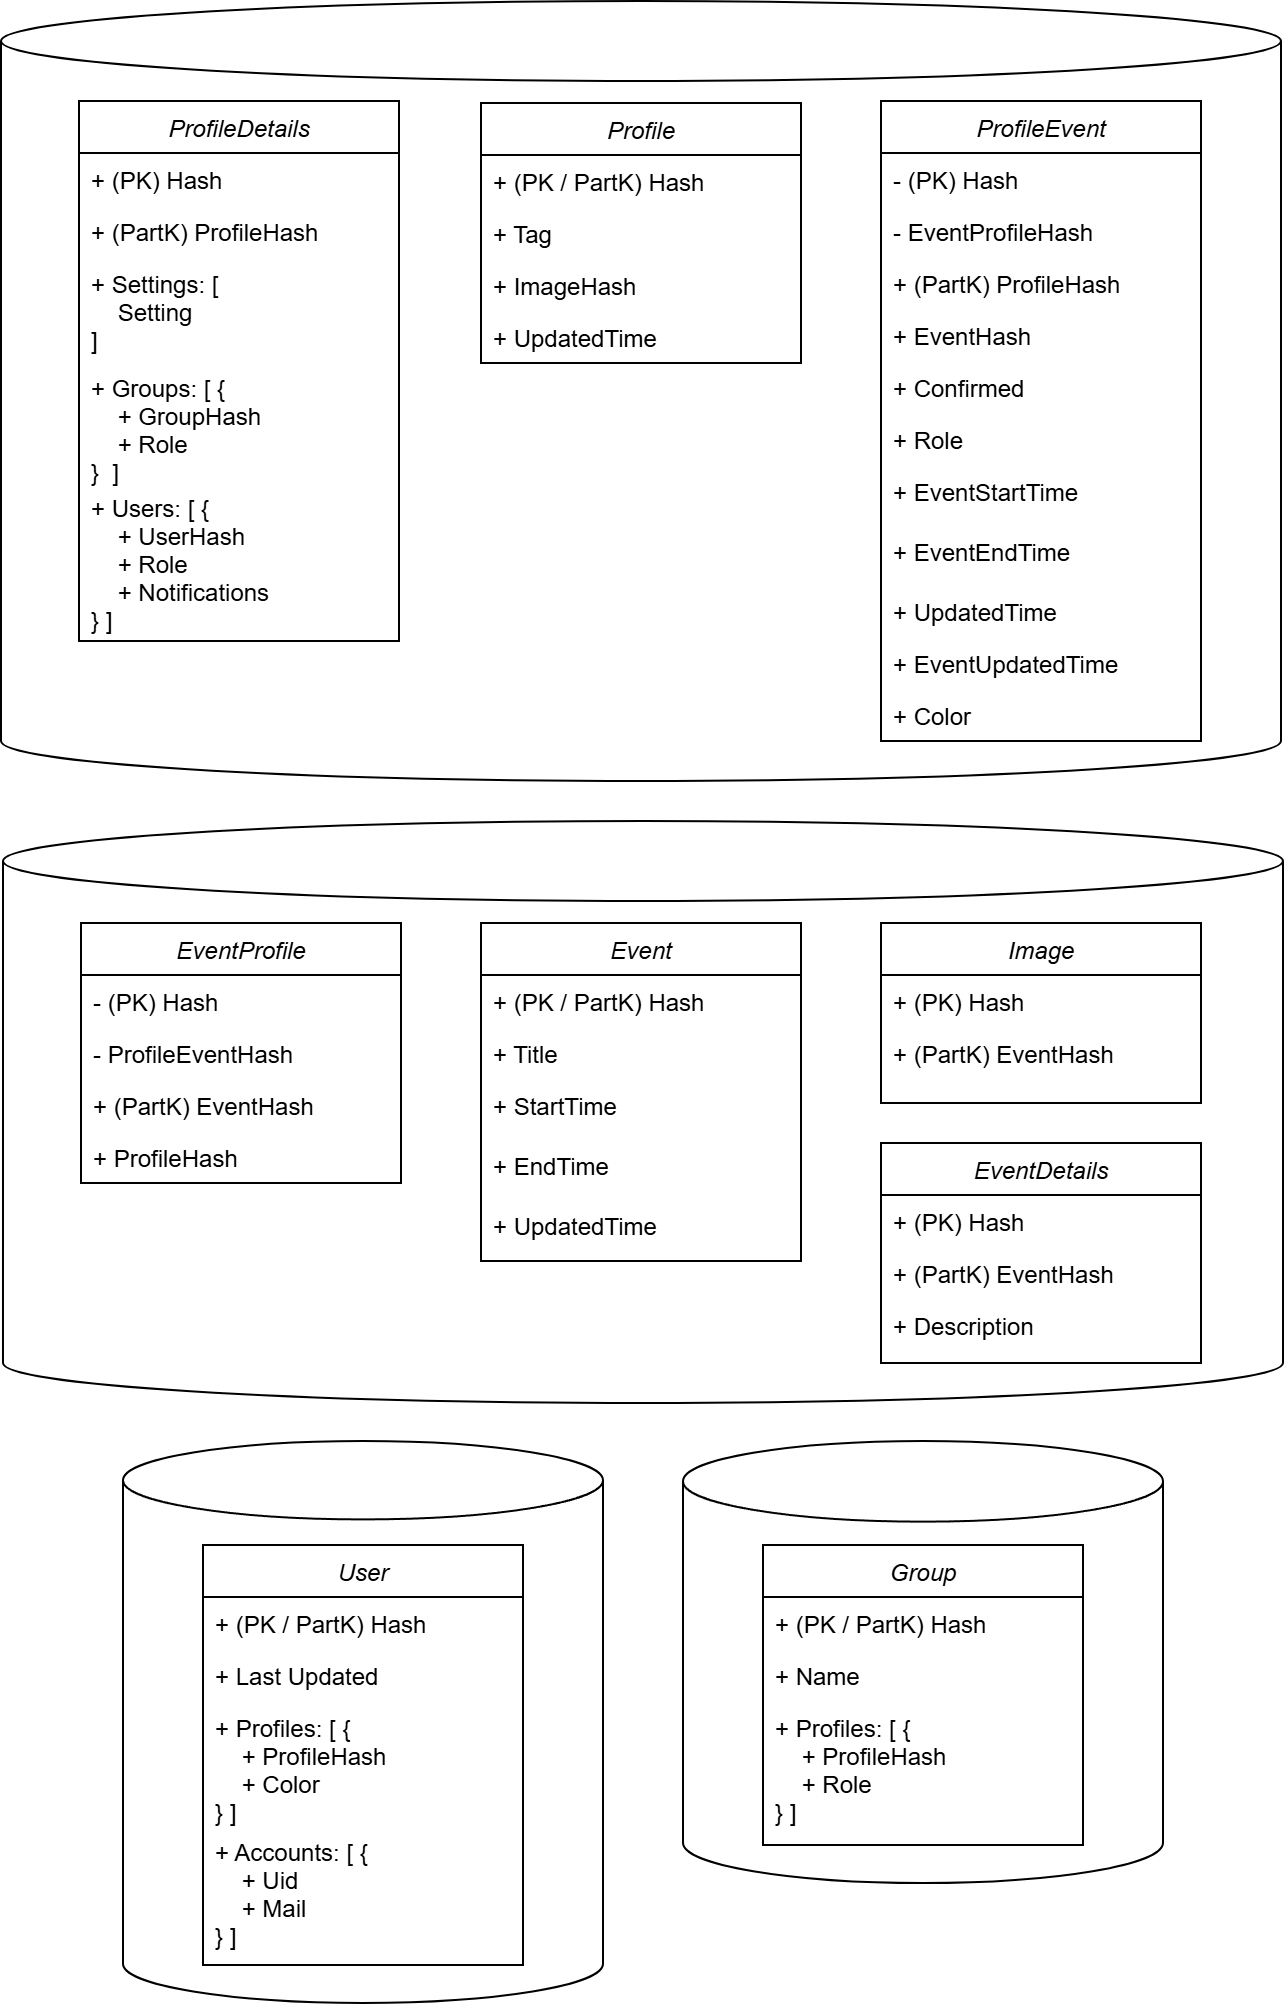
\includegraphics[height=.96\textheight]{NonRelationalModel.png}
    \caption{Modello delle collezioni e il loro partizionamento}
\end{figure}
\\
Allo stesso modo, laddove siano presenti relazioni uno a molti con cardinalità contenute,
è stato possibile integrarle all'interno degli oggetti stessi, duplicando i collegamenti.
Si evita così la necessità di cercare e recuperare i dati, 
rendendoli già direttamente disponibili.
È il caso di User e Profile, i quali contengono entrambi i corrispettivi riferimenti,
o delle immagini, in cui viene salvato il riferimento dell'Event in Image.
UserRole è stato integrato solo in ProfileDetails,
essendo necessario per controllare i permessi di un utente verso un profilo, e non il contrario.\\
\\
La relazione tra profili e gruppi vede invece cardinalità elevate:
non vi è un limite al numero di gruppi di cui un profilo può fare parte.
Non comportando dettagli particolari o interazioni complicate (in questa fase del progetto),
è stato considerato sufficiente mappare le relazioni
tramite liste all'interno di Group e ProfileDetails.\\
\\
Come analizzato nelle sezioni precedenti,
le richieste del progetto vertono sulla relazione tra eventi e profili.
In particolare, si prevede che le richieste più frequenti
(e quindi impattanti)
siano quelle di recupero dei dati generali su entrambi i versi della relazione
- eventi relativi ai profili o profili collegati agli eventi -
ma anche di conferma di un evento.
\clearpage
Vista la centralità delle richieste su queste entità,
sono state separate le proprietà di dettaglio da quelle essenziali,
salvandole in ProfileDetails ed EventDetails.
Oltre a migliorare il tempo di recupero delle informazioni
che si ritiene necessario essere immediatamente disponibili, 
si evita così che le operazioni che vertono su dati secondari 
impattino sul flusso principale delle richieste.
Riducendo la mole di dati da recuperare e analizzare,
si rendono le query relazionali meno pesanti e più veloci.\\
\\
Prevedendo che le richieste di conferma sullo stesso evento 
avvengano in momenti molto vicini tra loro,
si è deciso di non integrare la relazione nelle entità esistenti,
bensì di esternarla in documenti dedicati.
Si evita così di effettuare modifiche concorrenti sullo stesso Event.
Viene quindi introdotto ProfileEvent,
che presenta tutte le proprietà della relazione tra i due elementi.
Venendo partizionato in base all'hash del profilo corrispondente,
assolve il compito di recuperare gli eventi associati al profilo.
Include quindi il collegamento all'evento e
la conferma o meno della partecipazione del profilo all'evento,
ma anche la data dell'ultimo aggiornamento dell'evento associato,
in modo da consentire di controllare direttamente
se un evento è stato modificato rispetto all'ultimo aggiornamento,
e deve quindi essere caricato.\\
\\
Si prevede però che la quantità di richieste sia comunque importante
anche dal lato opposto della relazione,
ovvero per ottenere i profili correlati agli eventi.
Da un punto di vista prestazionale, 
non è accettabile che una ricerca attraversi le partizioni per recuperare queste informazioni.
Per questo motivo viene creato EventProfile,
che, partizionato assieme agli eventi,
mantiene le informazioni minime necessarie per ricondurre ai profili a esso collegati,
in maniera da limitare la quantità di dati da mantenere consistente.\\
\\
La distribuzione dei dati supporta così la totale scalabilità del sistema.
Ogni richiesta di dati infatti non incrocia mai più di tre elementi,
e in ogni caso possiede le informazioni relative alla partizione in cui il dato risiede.
Lo stesso può essere affermato per le richieste di modifica, 
che vertono su un unico elemento principale considerato come fonte di verità,
in base al quale le eventuali copie dovranno essere aggiornate.
Se è vero che le richieste sono state rese rapide 
sia in lettura che in scrittura,
la denormalizzazione che lo ha reso possibile
deve però prevedere un procedimento per l'allineamento dei dati copiati.
\clearpage

\subsection{Integrazione con le Azure Functions nel framework .Net}

L'utilizzo di un database documentale comporta
scelte implementative specifiche.
Il polimorfismo dei documenti e la denormalizzazione delle entità
rendono la rappresentazione logica degli elementi
e la loro relazione reciproca di secondaria importanza.
L'approccio a oggetti del Framework .Net assume quindi minore rilevanza,
in quanto si rende meno necessaria la capacità di descrivere e astrarre
le entità logiche attraverso classi di codice.
Si distinguono però due tipologie di richieste principali,
che determinano l'approccio apportato verso i dati:
la recupera di un elemento e la sua modifica.\\
\\
Quando è necessario recuperare un elemento dal database
risulta comodo convertirlo in un oggetto.
Questo consente di gestire le informazioni attraverso un'astrazione logica,
con tutti i relativi vantaggi.
La sua utilità risalta sopratutto nel caso in cui la lettura dell'elemento
non ha il solo fine di essere restituito al richiedente,
ma deve venire analizzato per procedere con la logica applicativa.
La rappresentazione dei documenti in oggetti 
crea infatti un codice più pulito e ordinato,
interagendo con le proprietà e i metodi della classe,
nascondendo la complessità computazionale dell'elaborazione del documento.
La conversione viene svolta automaticamente dal framework
e permette di associare ai dati il codice strettamente relativo, creando metodi appositi.\\
\\
Ogni elemento del dominio avrà quindi una classe associata,
con tutti i campi previsti dal modello.
Il contesto logico così introdotto agevola l'interazione tra i servizi e gli oggetti,
riducendo la probabilità di errori e semplificandone l'individuazione.
Anche il testing viene favorito, dando la possibilità di analizzare il codice
senza la necessità di interrogare il database o di simularlo.
Permette inoltre di automatizzare la conversione dei dati verso i DataTransferObject(DTO),
necessari per uniformare le risposte verso i client,
che contribuiscono a separare la logica di business da quella che gestisce la comunicazione.\\
\\
Nel caso la richiesta richieda invece la modifica di un elemento
la conversione del documento in oggetto risulta poco efficiente.
La creazione di un nuovo oggetto comporta infatti l'intera lettura dell'elemento associato.
Questo può essere utile se è necessario mantenere un riferimento logico,
per usare le informazioni che contiene
o per restituire al mittente l'oggetto aggiornato.
Nella maggior parte dei casi si vuole invece semplicemente applicare una modifica,
lasciando che sia il sistema a portarla a compimento.
In tal caso, Cosmos DB permette le cosiddette patch update,
ovvero modifiche limitate al campo interessato,
che non richiedono la lettura e la sovrascrittura dell'intero documento.
Per queste occasioni vengono implementati appositi metodi che,
presi in ingresso i dati da modificare,
interagiscono con il database per aggiornare le sole parti coinvolte.\\
\\
La comunicazione con il database viene astratta tramite un servizio dedicato chiamato WydDbService.
WydDbService ha il compito di gestire le richieste e le sessioni con il database,
nascondendo le complessità implementative e di interazione.
In particolare, la connessione con il database comporta
la richiesta verso Azure Key Vault per il recupero delle chiavi di accesso,
per poi usarle per stabilire un canale attraverso il quale applicare le modifiche.
Mette inoltre a disposizione un'interfaccia per nascondere
tutte le logiche di basso livello dovute dall'interazione specifica di CosmosDB.
Verrà utilizzato dagli altri servizi tramite dependency injection,
automatizzandone la creazione e l'utilizzo,
e di conseguenza la connessione e le richieste al database.

\subsection{Garantire la consistenza finale dei dati}

Avendo salvato le entità del dominio sotto forma di documenti denormalizzati,
la modifica del campo di un elemento potrebbe dover comportare
la necessità di propagare gli aggiornamenti 
su tutti gli altri componenti in cui tale dato è duplicato.
Potendo accettare un ritardo nell'allineamento dei dati,
è possibile separare la modifica del documento principale
dalla sua distribuzione sul resto del database.\\
\\
Affidare il compito di aggiornare tutti i componenti secondari coinvolti
alla stessa funzione risulta svantaggioso sotto molti aspetti.
Si introdurrebbe infatti un ritardo nell'esecuzione,
dovuto all'attesa della conclusione delle ulteriori modifiche,
che devono essere controllate e gestite in caso falliscano.
Complicare la funzione va inoltre contro
i principi stessi dei servizi serverless,
che prevedono invece strutture semplici con responsabilità precise e limitate.
La loro efficienza deriva infatti dalla possibilità
di eseguire in maniera autonoma compiti specifici.
L'unico requisito necessario per permettere a una funzione
di delegare ad altre le modifiche derivate
è la garanzia che la loro esecuzione venga controllata e
che quindi venga assicurato il un loro eventuale successo.
\clearpage
L'introduzione di una funzione con il ruolo di orchestratore
non sposterebbe di molto il problema.
Nonostante soddisfi la necessità di affidare a diverse funzioni
le diverse parti del problema e sia in grado di controllarne il risultato,
- potendone così garantire il successo -
implica comunque l'attesa del loro completamento.
Aggiungerebbe inoltre un ritardo dovuto al tempo necessario per la sua stessa esecuzione,
che aspetta e controlla le funzioni che ha chiamato.
Questo ritardo è negativamente influenzato dall'accoppiamento debole
tra l'orchestratore e le funzioni figlie,
che non assicura l'immediata ripresa del padre 
al termine dell'esecuzione di una funzione da lui chiamata.
Le dipendenze che verrebbero così introdotte tra 
l'orchestratore, la funzione originale e quelle necessarie per la consistenza dei dati
comporterebbero solo rischi di fallimento e l'allungamento dei tempi di risposta.\\
\\
A questo scopo,
Azure Cosmos DB mette a disposizione uno strumento apposito, chiamato Change Feed.
Change Feed è un meccanismo tramite il quale è possibile
associare le modifiche di un elemento del database
all'esecuzione di una funzione.
Il Change Feed viene definito come trigger all'interno di una funzione,
e viene associato a una collezione di documenti.
Ogni volta che un documento di questa collezione subisce un aggiornamento
si crea in automatico un log che,
all'interno della stessa partizione coinvolta,
viene salvato in una nuova collezione dedicata chiamata "lease".
Change Feed è dunque il meccanismo che,
nel momento in cui un log viene aggiunto alla sua lease,
fa partire autonomamente la funzione associata.\\
\\
La funzione, una volta invocata,
legge dal lease tutti i log che non sono ancora stati processati,
per poi propagare le modifiche ove necessario.
L'avvenuto successo dell'elaborazione del log viene registrato
grazie a dei token di aggiornamento,
che permettono di sapere in quale punto del lease 
sono presenti i log che non sono ancora stati processati.
La persistenza dei log sui lease garantisce
che la modifica sia presa in carico da una funzione almeno una volta,
mentre la presenza dei token di aggiornamento assicura
che la funzione venga eseguita di nuovo in seguito a un errore o a un guasto del sistema,
soddisfando così i requisiti di invocazione.
Questo meccanismo è intrinsecamente scalabile.
Essendo infatti i lease associati alle partizioni in cui risiedono i documenti,
è possibile dividere (e quindi distribuire, quando necessario) il carico su più funzioni.\\
\\
Il Change Feed viene usato, ad esempio,
nel caso in cui venga cambiata un'informazione importante di un evento.
Questa operazione comporta l'aggiornamento di UpdatedDate,
campo che memorizza il momento in cui è stata apportata l'ultima modifica.
UpdatedDate è stata denormalizzata all'interno dei ProfileEvent,
e la sua modifica deve essere quindi propagata.
La propagazione di questo aggiornamento sarà delegata a una seconda funzione.
L'invocazione di questa funzione verrà associata
al lease relativo alla collezione degli Event,
nel caso siano presenti log non ancora elaborati.\\
\\
In questa maniera i compiti vengono efficacemente suddivisi in due funzioni,
indipendenti tra loro.
La prima funzione avrà il solo compito di cambiare la proprietà dell'oggetto,
informando il client riguardo al successo dell'operazione.
Una seconda funzione, attivata in autonomia dal Change Feed,
si occuperà poi di aggiornare tutti i ProfileDetails relativi,
senza andare a impattare sulle prestazioni o sulle dipendenze della prima.\\
\begin{figure}[htbp]
    \centering
    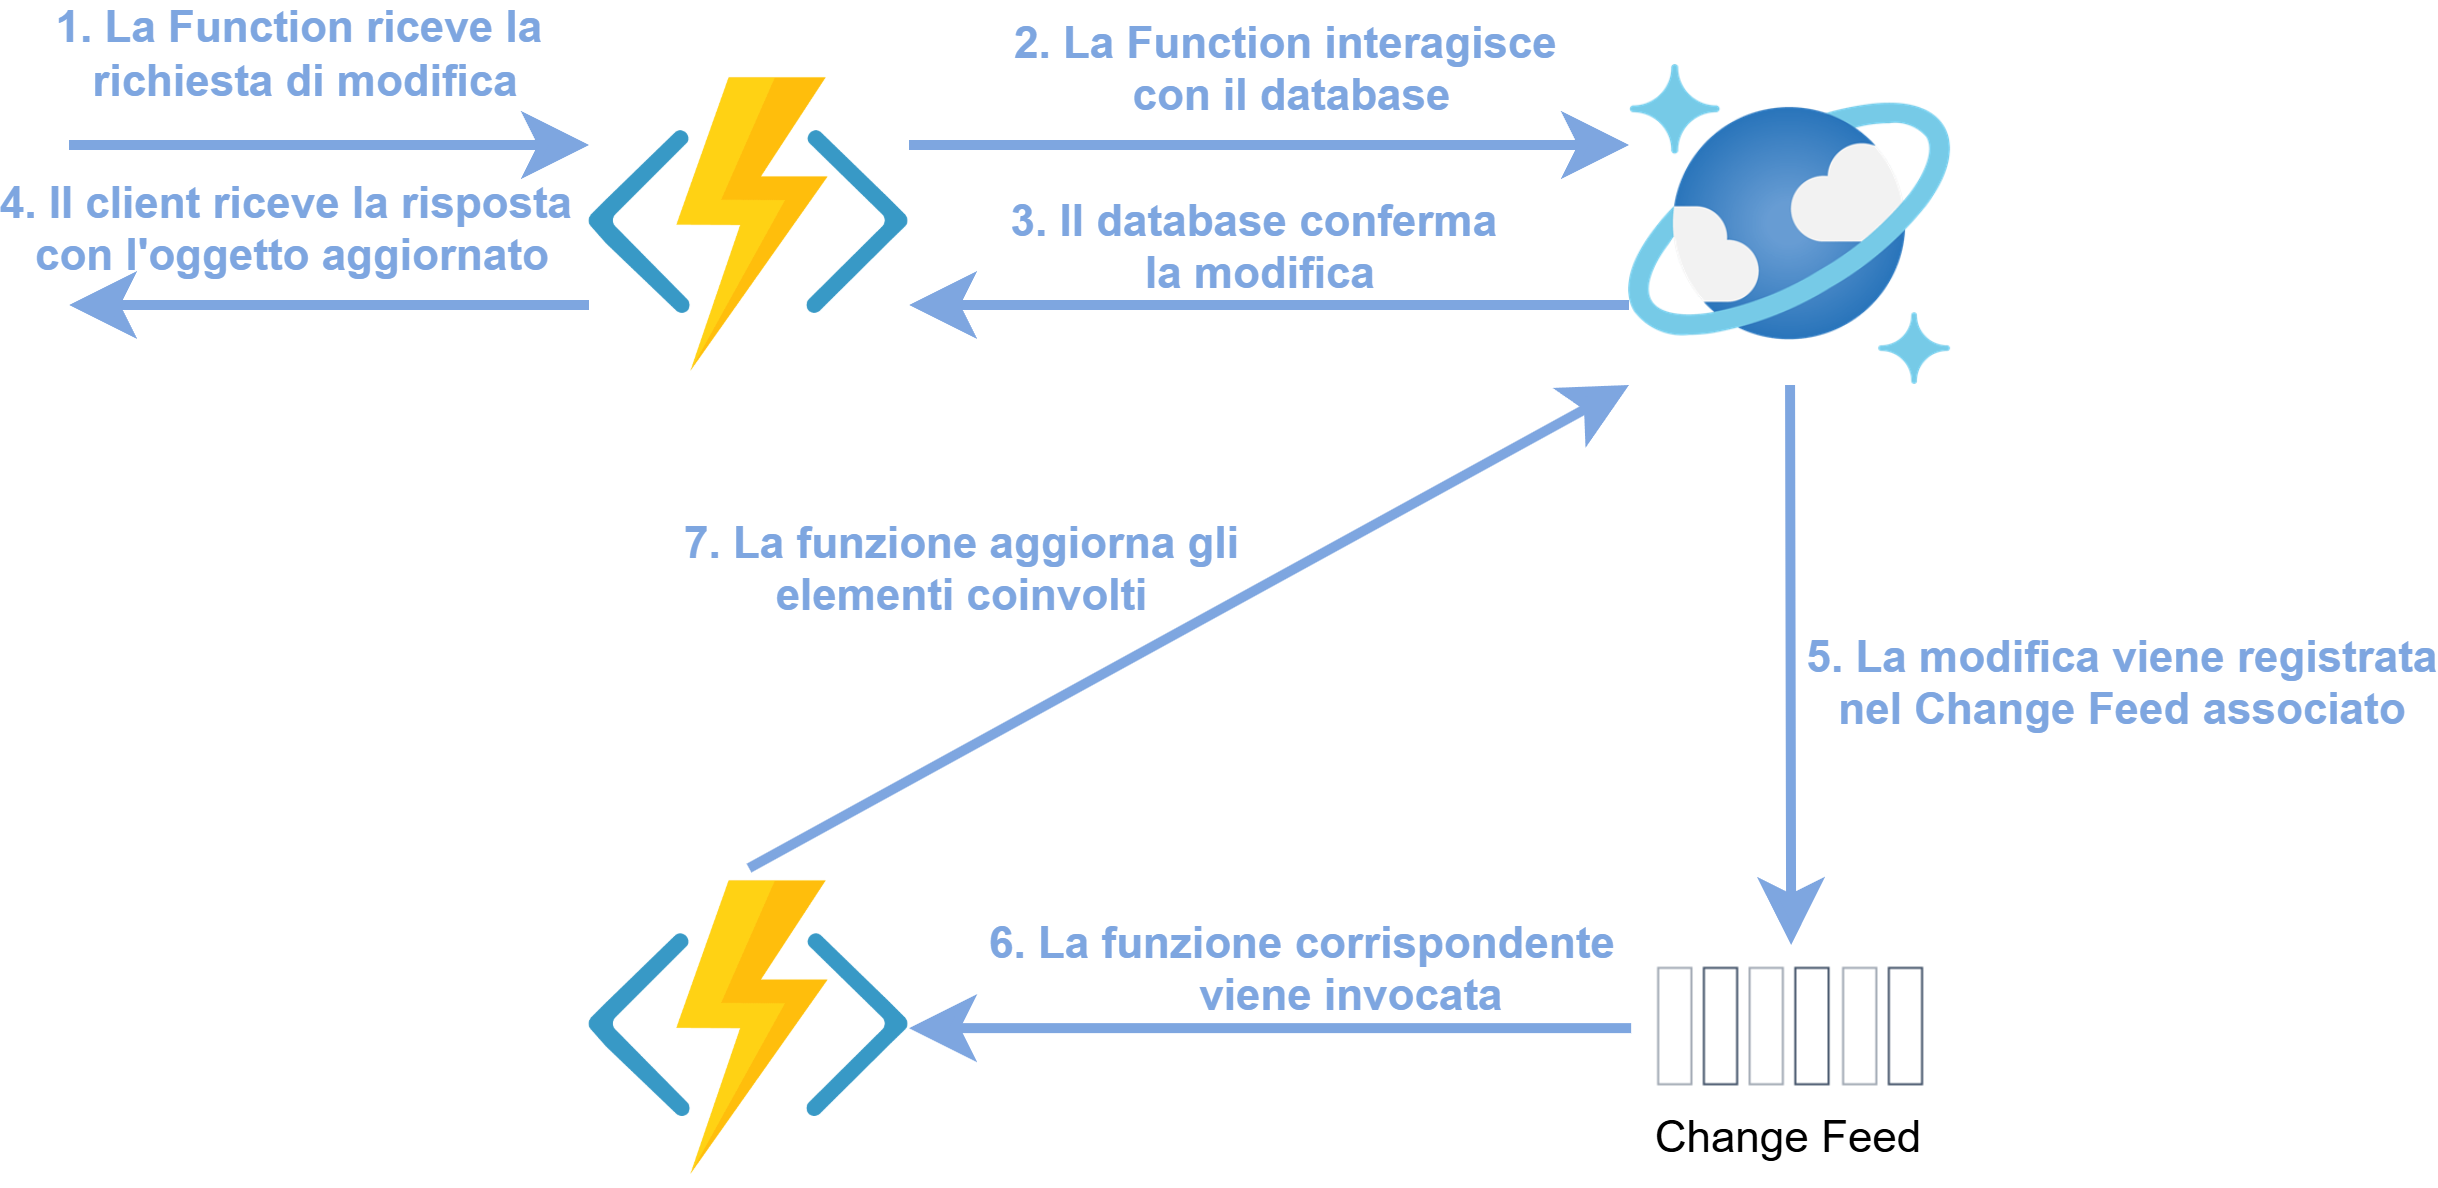
\includegraphics[width=\textwidth]{EventChangeFeed.png}
    \caption{Aggiornamento dei documenti tramite Change Feed}
\end{figure}
\\
Ci sono situazioni in cui il Change Feed non può essere usato.
È ad esempio il caso della conferma di un evento.
L'elemento primario coinvolto in questa operazione è ProfileEvent,
che sarà modificato dalla funzione iniziale.
La conferma di partecipazione a un evento da parte di un profilo
viene considerato come modifica all'evento stesso,
che comporta quindi l'aggiornamento del documento Event.
Se però si associasse una funzione anche per le modifiche a ProfileEvent tramite Change Feed,
si verrebbe a creare una ricorsione infinita per il quale 
la modifica a un ProfileEvent comporta la modifica a un Event, 
che a sua volta comporta una modifica a ProfileEvent, e via dicendo.\\
\\
Per quanto sia possibile aggiungere all'interno delle funzioni controlli
che analizzino ogni volta l'origine della richiesta,
questo porterebbe a una maggiore complessità e a un aumento del carico implementativo,
introducendo nuovi dati all'interno di ogni aggiornamento.
Si è quindi deciso di utilizzare il ChangeFeed solo per le entità
la cui modifica influenza molteplici altri documenti,
delegando in maniera differente l'eventuale aggiornamento di un altro elemento singolo.\\
\\
Esistono diversi altri strumenti che le Azure Functions possono sfruttare
per invocare in maniera asincrona un'altra funzione, senza passare per l'utilizzo di un orchestratore.\\
\\
Una prima soluzione può essere l'invio di una nuova richiesta HTTP al server stesso,
al quale è associata la funzione voluta.
Per quanto risulti veloce e facile da implementare,
questa soluzione non garantisce l'effettiva
presa in carico, esecuzione e completamento della richiesta,
a meno di controllarne la risposta.
Il controllo della risposta comporta però l'attesa della richiesta,
procedimento che mina la finalità stessa dell'operazione.\\
\\
Azure mette invece a disposizione servizi basati su code ed eventi
proprio per mettere in comunicazione diverse parti di uno stesso sistema.
Tra le funzionalità offerte da Azure e
quindi direttamente integrabili con le Azure Functions troviamo
Azure Queue Storage, Azure Service Bus e Azure Event Hub.\\
\\
Azure Queue Storage è un servizio di code di messaggi
offerto come parte di Azure Storage,
che si occupa del salvataggio di informazioni
che non rientrano nei casi d'uso dei database tradizionali.
Le funzioni hanno quindi la possibilità di aggiungere alla coda i propri messaggi,
che verranno poi elaborati da un'altra funzione grazie a un trigger associato.
La dimensione massima che i messaggi possono avere è 64 Kb,
e rimangono in memoria per un tempo prestabilito, che può essere configurato.
Le code sono persistenti e altamente disponibili,
assicurando che i messaggi non vadano persi in caso di fallimento del consumer,
ma non presentano ulteriori funzionalità associate.
\clearpage

La sua semantica di consegna garantisce che il messaggio venga elaborato almeno una volta,
il che significa che la sua consegna potrebbe avvenire più volte,
nel caso in cui a prima funzione che lo prende in carico
termini con errori o raggiunga il timeout di elaborazione.
Presenta quindi un servizio semplice e veloce,
estremamente robusto ma anche scalabile.
La sua semplicità, sebbene contribuisca a ridurne il costo,
ne comporta però la mancanza di ulteriori proprietà avanzate.
Ad esempio, Azure Queue Storage non presenta la capacità
di gestire i messaggi in caso la loro esecuzione continui a fallire,
caratteristica che può essere desiderata in caso sia necessario assicurare
che l'operazione giunga al suo termine.\\
\\
Azure Service Bus è invece un servizio di messaggistica
che supporta scenari più complessi rispetto a Queue Storage.
Offre due tipologie principali di comunicazione: code e argomenti.
Le code di Service Bus supportano le stesse funzionalità del servizio precedente,
a cui però se ne aggiungono di più avanzate quali l'ordinamento,
le sessioni per il raggruppamento di messaggi correlati,
la funzionalità di "dead-letter queue" integrata
(per la gestione automatica dei messaggi non elaborabili) e
l'elaborazione transazionale.\\
\\
Gli argomenti (topics) prevedono un pattern publish/subscribe,
nel quale più fruitori possono collegarsi allo stesso argomento per poi
venire tutti notificati in contemporanea in caso venga inviato un messaggio a esso inerente.
Essendo stato progettato per soddisfare carichi di lavoro a livello aziendale,
garantisce un'elevata scalabilità,
oltre a fornire assicurazioni di consegna più robuste e
integrare meccanismi di gestione degli errori.
Risulta però più costoso e relativamente più complesso da utilizzare.\\
\\
Azure Event Hub è un servizio di ingestione di dati altamente scalabile e a bassa latenza,
progettato per lo streaming di grandi volumi di eventi da diverse fonti.
Non è una coda di messaggi nel senso tradizionale,
ma piuttosto un "broker di eventi",
in cui gli eventi vengono aggiunti a una coda distribuita su più partizioni,
dove rimangono disponibili per i consumer per un periodo configurabile (fino a 90 giorni).
I consumer leggono gli eventi dalla partizione mantenendo ognuno il proprio progresso,
il che permette a più consumer group di leggere gli stessi eventi indipendentemente.
Anche in questo caso, la semantica garantisce che il messaggio venga elaborato almeno una volta.
\clearpage
Presenta quindi elevate caratteristiche di scalabilità,
fornendo una bassa latenza, un throughput estremamente elevato
e la possibilità di parallelizzare il consumo dei messaggi.
Pur mantenendo in memoria i dati
- e quindi assicurando che sia sempre possibile applicare le modifiche -
tutta la logica necessaria per controllare l'esecuzione, ritentare ed eliminare il messaggio
rimane però a carico dello sviluppatore.\\
\begin{longtable}{|P{2.9cm}|P{3.9cm}|P{3.9cm}|P{3.9cm}|}
    \hline
    \textbf{Caratteristica} & \textbf{Queue Storage}                                         & \textbf{Service Bus}                                                              & \textbf{Event Hub}                                                      \\
    \hline
    Tipo di servizio        & Coda di messaggi semplice                                      & Coda/Broker di messaggi                                                           & Flusso di eventi                                                        \\
    \hline
    Modalità di fruizione   & Competing Customers (Point-to-point)                           & Competing Customers (Point-to-point)\newline Publish/Subscribe (argomenti)        & Publish/ Subscribe (molti a molti)                                      \\
    \hline
    Caratteristiche         & Semplice, scalabile e robusto ma nessun controllo degli errori & Affidabile, scalabile, garantisce il controllo dell'esecuzione, ordina i messaggi & Scalabile, robusto, ordinato ma nessun controllo sull'esecuzione        \\
    \hline
    Costo                   & €0,04 GB/mese + €0.0004 ogni diecimila operazioni              & €0,044 ogni milione di operazioni (piano Basic con solo le code)                  & €0,014/ora per ogni Unità di throughput + €0,025 ogni milione di eventi \\
    \hline
    \caption{Proprietà dei servizi Azure per la propagazione interna di messaggi }
\end{longtable}


Viste queste considerazioni,
per garantire la consistenza degli oggetti 
nei casi in cui non sia possibile sfruttare il Change Feed
si è scelto di adottare Azure Service Bus.
\begin{wrapfigure}{o}{0.25\textwidth}
    \centering
    
\includegraphics[height=.12\textheight]{servicebus.png}
    Service Bus
\end{wrapfigure}
La scelta deriva principalmente dal supporto nativo
al controllo dell'esecuzione delle funzioni,
grazie all'utilizzo delle dead-letter queue.
Una dead-letter queue è un contenitore in cui vengono inseriti
tutti i messaggi la cui elaborazione è stata tentata e fallita una determinata quantità di volte.
Garantisce quindi, in aggiunta a ulteriori tentativi in caso di insuccesso,
il monitoraggio di tutte le operazioni che non riescono a essere portate a termine.
Questo permette di assicurare che gli aggiornamenti necessari per allineare i documenti
siano sempre controllati.\\
\\
Tornando all'esempio precedente
- nel quale era necessario propagare la conferma di un evento -
la modifica di Event e di EventProfile verrà eseguita da due funzioni dedicate.
Al termine della modifica di ProfileEvent,
la funzione inserirà in coda al Service Bus un messaggio
con le informazioni necessarie alle altre due,
per poi inviare la risposta al client.
Le due funzioni verranno quindi invocate,
aggiornando gli elementi coinvolti.
Nel caso di Event, il Change Feed associato aggiornerà di conseguenza
tutti i sui ProfileEvent, senza però creare ricorsioni.\\

\begin{figure}[h!]
    \centering
    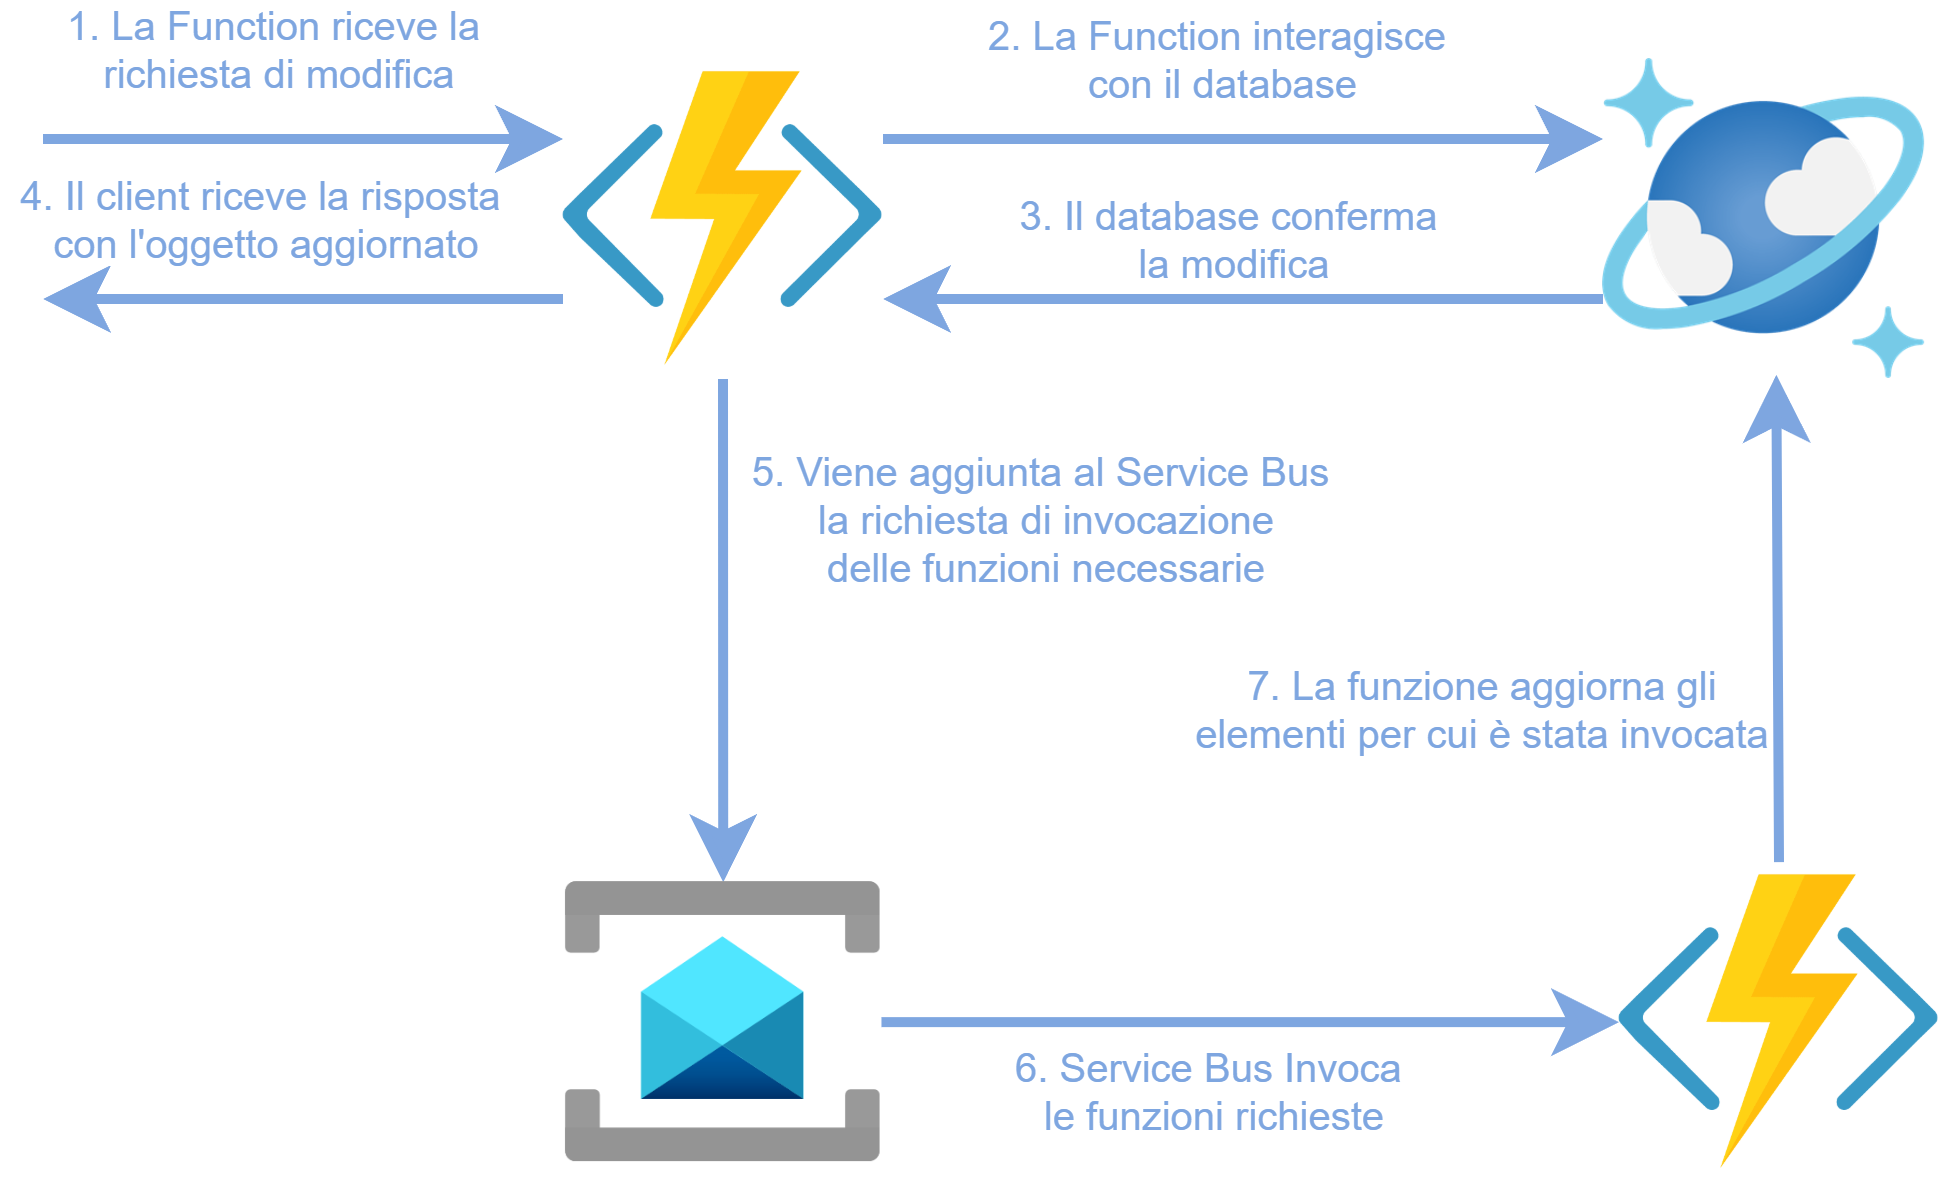
\includegraphics[height=0.39\textheight]{EventServiceBus.png}
    \caption{Fasi di aggiornamento tramite Service Bus}
\end{figure}




\clearpage